\begin{figure}[H]
\centering
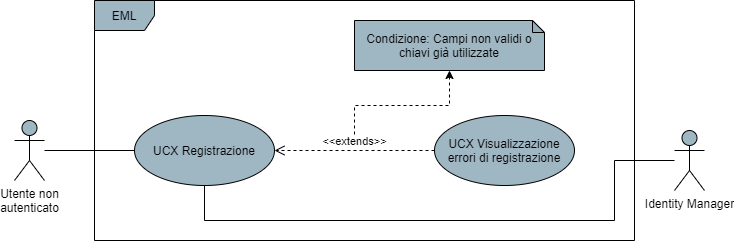
\includegraphics[scale=0.6]{res/UseCase/Immagini/RegistrazioneGenerale}
\caption{Schema generale: modulo di registrazione cliente}
\end{figure}

\subsubsection{UC1 - Registrazione cliente}
\begin{itemize}
\item \textbf{Attori primari}: utente non autenticato;
\item \textbf{Attori secondari}: Identity Manager;
\item \textbf{Descrizione}: viene effettuata la registrazione di un cliente nel sistema, inserendo i propri dati personali nella pagina dedicata;
\item \textbf{Scenario Principale}: l'utente non autenticato accede alla pagina di registrazione, il sistema rende disponibili i campi da compilare, l'utente compila i campi [\textbf{UC1.1}], conferma la registrazione [\textbf{UC1.2}] e l'Identity Manager si occupa della registrazione dell'utente nel sistema;
\item \textbf{Estensioni}:
\begin{itemize}
\item \textbf{UC2}: se i campi non sono validi o l'email è già stata utilizzata nel sistema, viene mostrato un errore di registrazione all'utente non autenticato che potrà provare nuovamente ad eseguire la registrazione.
\end{itemize}
\item \textbf{Precondizione}: l'utente non autenticato intende registrarsi nel sistema come cliente;
\item \textbf{Postcondizione}: l'utente risulta registrato nel sistema come cliente.
\end{itemize}

\begin{figure}[H]
\centering
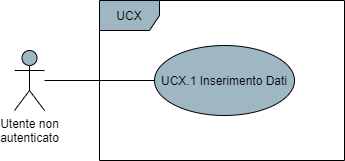
\includegraphics[scale=0.6]{res/UseCase/Immagini/Registrazione}
\caption{Diagramma UML\ped{G} per UC1 - Registrazione cliente}
\end{figure}

\subsubsection{UC1.1 - Inserimento dati}
\begin{itemize}
\item \textbf{Attori primari}: utente non autenticato;
\item \textbf{Descrizione}: l'utente compila il form per la registrazione nel sistema;
\item \textbf{Scenario Principale}: l'utente inserisce i seguenti dati personali:
\begin{itemize}
\item nome [\textbf{UC1.1.1}];
\item cognome [\textbf{UC1.1.2}];
\item indirizzo di fatturazione [\textbf{UC1.1.3}];
\item email [\textbf{UC1.1.4}];
\item password [\textbf{UC1.1.5}].
\end{itemize}
\item \textbf{Precondizione}: l'utente non autenticato è all'interno della pagina di registrazione;
\item \textbf{Postcondizione}: l'utente ha compilato tutti campi e può procedere alla registrazione.
\end{itemize}

\begin{figure}[H]
\centering
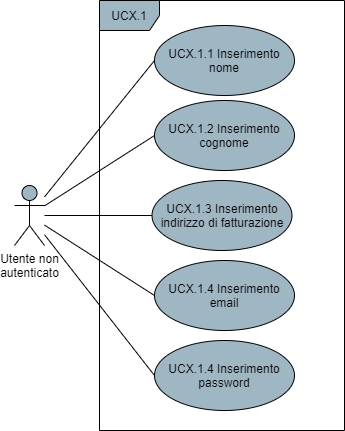
\includegraphics[scale=0.6]{res/UseCase/Immagini/InserimentoDatiRegistrazione}
\caption{Diagramma UML\ped{G} per UC1.1 - Inserimento dati}
\end{figure}


\subsubsection{UC1.1.1 - Inserimento nome}
\begin{itemize}
\item \textbf{Attori primari}: utente non autenticato;
\item \textbf{Descrizione}: l'utente deve compilare il campo ``Nome" per procedere alla registrazione;
\item \textbf{Scenario Principale}: l'utente inserisce il suo nome nell'apposito campo;
\item \textbf{Precondizione}: il campo ``Nome" risulta vuoto;
\item \textbf{Postcondizione}: il campo ``Nome" è stato compilato.
\end{itemize}

\subsubsection{UC1.1.2 - Inserimento cognome}
\begin{itemize}
\item \textbf{Attori primari}: utente non autenticato;
\item \textbf{Descrizione}: l'utente deve compilare il campo ``Cognome" per procedere alla registrazione;
\item \textbf{Scenario Principale}: l'utente inserisce il suo cognome nell'apposito campo;
\item \textbf{Precondizione}: il campo ``Cognome" risulta vuoto;
\item \textbf{Postcondizione}: il campo ``Cognome" è stato compilato.
\end{itemize}

\subsubsection{UC1.1.3 - Inserimento indirizzo di fatturazione}
\begin{itemize}
\item \textbf{Attori primari}: utente non autenticato;
\item \textbf{Descrizione}: l'utente deve compilare il campo ``Indirizzo di fatturazione" per procedere alla registrazione;
\item \textbf{Scenario Principale}: l'utente inserisce il suo indirizzo di fatturazione nell'apposito campo;
\item \textbf{Precondizione}: il campo ``Indirizzo di fatturazione" risulta vuoto;
\item \textbf{Postcondizione}: il campo ``Indirizzo di fatturazione" è stato compilato.
\end{itemize}

\subsubsection{UC1.1.4 - Inserimento email}
\begin{itemize}
\item \textbf{Attori primari}: utente non autenticato;
\item \textbf{Descrizione}: l'utente deve compilare il campo ``Email" per procedere alla registrazione;
\item \textbf{Scenario Principale}: l'utente inserisce la sua email nell'apposito campo;
\item \textbf{Precondizione}: il campo ``Email" risulta vuoto;
\item \textbf{Postcondizione}: il campo ``Email" è stato compilato.
\end{itemize}

\subsubsection{UC1.1.5 - Inserimento password}
\begin{itemize}
\item \textbf{Attori primari}: utente non autenticato;
\item \textbf{Descrizione}: l'utente deve compilare il campo ``Password" per procedere alla registrazione;
\item \textbf{Scenario Principale}: l'utente inserisce una password nell'apposito campo;
\item \textbf{Precondizione}: il campo ``Password" risulta vuoto;
\item \textbf{Postcondizione}: il campo ``Password" è stato compilato.
\end{itemize}

\subsubsection{UC1.2 - Conferma registrazione}
\begin{itemize}
\item \textbf{Attori primari}: utente non autenticato;
\item \textbf{Descrizione}: l'utente conferma i dati presenti nel form e si registra nel sistema;
\item \textbf{Scenario Principale}: l'utente preme il tasto di conferma di registrazione e manda la richiesta al sistema per la registrazione di un account con i dati presenti nel form;
\item \textbf{Precondizione}: l'utente non autenticato si trova all'interno della pagina di registrazione;
\item \textbf{Postcondizione}: la richiesta di registrazione è stata mandata al sistema.
\end{itemize}

\subsubsection{UC2 - Visualizzazione errori di registrazione}
\begin{itemize}
\item \textbf{Attori primari}: utente non autenticato;
\item \textbf{Descrizione}: l'utente non autenticato visualizza un errore riguardante i campi di registrazione che ha inserito. Questi errori possono essere:
\begin{itemize}
\item \textbf{Campo non valido}: un campo risulta vuoto o con caratteri non validi;
\item \textbf{Email già utilizzata}: l'email è già stata utilizzata da un altro cliente.
\end{itemize}
\item \textbf{Scenario Principale}: il sistema riconosce uno o più errori nei campi inseriti dall'utente e vengono visualizzati nella pagina di registrazione;
\item \textbf{Precondizione}: l'utente non autenticato ha inserito i campi ed ha provato ad effettuare la registrazione;
\item \textbf{Postcondizione}: viene visualizzato un messaggio di errore nella pagina di registrazione e l'utente non risulta autenticato nel sistema.
\end{itemize}

